\documentclass[aspectratio=169]{beamer}
\usepackage[utf8]{inputenc} % codificacao de caracteres
\usepackage[T1]{fontenc}    % codificacao de fontes
%\usepackage[brazil]{babel}  % idioma
\usepackage{graphics,amssymb,amsfonts,amsmath}
\usepackage{tikz}
\usepackage{enumerate,hyperref}
\usepackage{palatino}	% Fonte sem serifa
\usepackage{ragged2e}	% Paragrafo justificado
%\usepackage{minted}	% Highlight para codigos de programacao
\usepackage{booktabs} % tabelas

% Veja mais temas e cores em http://www.hartwork.org/beamer-theme-matrix/
\usetheme{Montpellier}         % tema
\usecolortheme{orchid}      % cores
\usefonttheme[onlymath]{serif} % fonte modo matematico
% Colocando numero de paginas no slide
\setbeamertemplate{footline}[frame number]



\DeclareGraphicsExtensions{.pdf,.JPG,.JPG} % compilamos apenas com pdflatex
\graphicspath{{./figuras/}} % caminho onde as figuras estarao disponiveis




% ---------------------------------------------------------------------------- %
% T�tulo                                                                       %
% ---------------------------------------------------------------------------- %

\title[\sc{Teoria de Circuitos Eletrônicos 1}]{\LARGE Aula 1: Resistive Circuits}
\author[Prof. Marcelino Andrade]{Prof. Marcelino Andrade}
\institute{Faculdade UnB Gama} % opcional
\date{\today}

\begin{document}
\justifying % Paragrafo justificado
\pagebreak

\begin{frame}
  \titlepage
\end{frame}


% ----------------- NOVO SLIDE --------------------------------
\begin{frame}{Contents}
\tableofcontents
\begin{center}	
     		Introduction to Electric Circuits 9th Edition by James A. Svoboda, Richard C. Dorf			
\end{center}	
\end{frame}

% ----------------- NOVA SECÇÂO -----------------------------
\section{Indroduction (3.1)}
% ----------------- NOVO SLIDE --------------------------------
\begin{frame}[fragile]
	\frametitle{Resistive Circuits}
		\begin{tabular}{ll}
			\begin{columns}
				\begin{column}{0.5\textwidth}  %%<--- here
    				%	\begin{figure}	
     					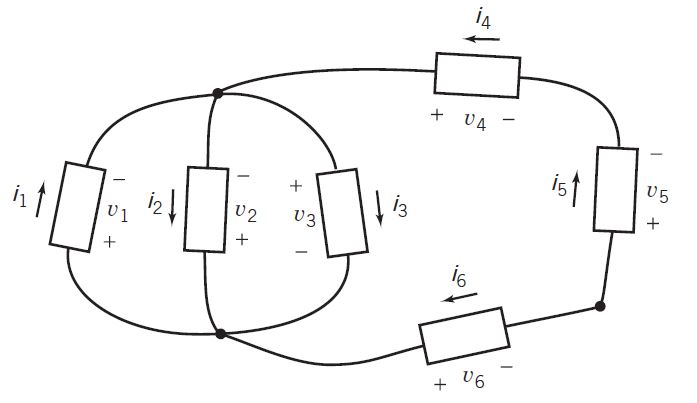
\includegraphics[width=.8\textwidth]{figura1.JPG}\\		
					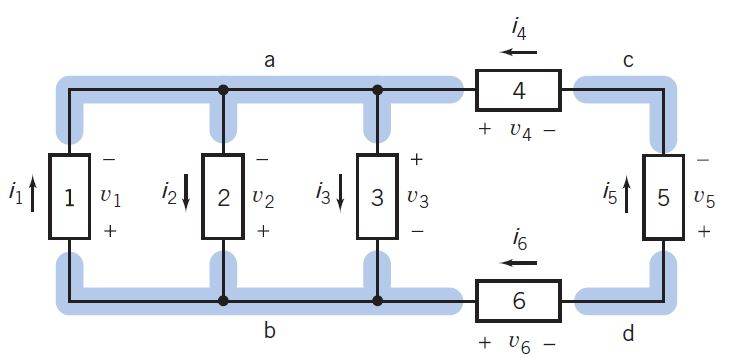
\includegraphics[width=.8\textwidth]{figura2.JPG}\\	
     				%	\end{figure}	
				\end{column}
				\begin{column}{0.5\textwidth}  %%<--- here
    					\begin{itemize}
						\item[$\clubsuit$] An electric circuit consists of circuit elements that are connected together.
						\item[$\clubsuit$] The same circuit can be drawn in several ways.							
						\item[$\clubsuit$] The places where the elements are connected to each other are called nodes.
					\end{itemize}
				\end{column}
			\end{columns}
		\\
			\begin{columns}[c]
				\column{1\textwidth}
		
			\end{columns}
		\end{tabular}
\end{frame}
% ----------------- NOVO SLIDE --------------------------------
\begin{frame}[fragile]
	\frametitle{Resistive Circuits}
		\begin{tabular}{ll}
			\begin{columns}[c]
				\column{1\textwidth}
				We say that circuit drawings A and B represent the same circuit when the following three conditions are met.		
			\end{columns}
		 \\
			\begin{columns}
				\begin{column}{0.3\textwidth}  %%<--- here
					\begin{tabular}{ll}
					%\begin{center}	
     						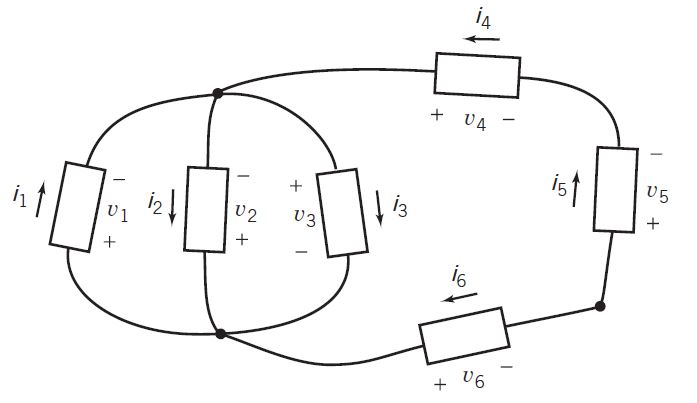
\includegraphics[width=1\textwidth]{figura1.JPG}(A)
						 \\
	     					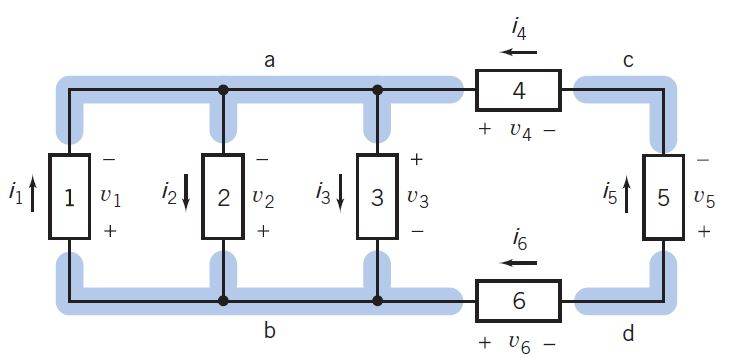
\includegraphics[width=1\textwidth]{figura2.JPG}(B)
					%\end{center}	
 					\end{tabular}
				\end{column}
				\begin{column}{0.7\textwidth}
					\begin{itemize}
						\item[$\clubsuit$] There is a one-to-one correspondence between the nodes of drawing A and the nodes of drawing B.
						\item[$\clubsuit$] There is a one-to-one correspondence between the elements of drawing A and the elements of drawing B.							
						\item[$\clubsuit$] Corresponding elements are connected to corresponding nodes.
					\end{itemize}
				\end{column}
			\end{columns}
		\end{tabular}
\end{frame}
% ----------------- NOVA SECÇÂO -----------------------------
\section{Kirchhoff’s Laws (3.2)}
% ----------------- NOVO SLIDE --------------------------------
\begin{frame}[fragile]
	\frametitle{Kirchhoff’s Laws}
		\begin{tabular}{ll}
			\begin{columns}[c]
				\column{1\textwidth}
				In 1847, Gustav Robert Kirchhoff, a professor at the University of Berlin, formulated
				two important laws that provide the foundation for analysis of electric circuits.
			\end{columns}
		 \\
			\begin{columns}
				\begin{column}{0.3\textwidth}  %%<--- here
    					\begin{center}	
     						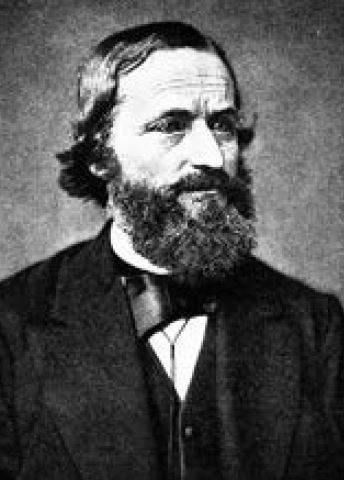
\includegraphics[width=.5\textwidth]{figura3.JPG}\\
     					\end{center}	
				\end{column}
				\begin{column}{0.8\textwidth}  %%<--- here
    					\begin{itemize}
						\item[$\clubsuit$] \textbf{Kirchhoff’s current law (KCL):} The algebraic sum of the currents into a node at any instant is zero.
						\item[$\clubsuit$] \textbf{Kirchhoff’s voltage law (KVL):} The algebraic sum of the voltages around any loop in a circuit is identically zero for all time.	
					\end{itemize}
				\end{column}
			\end{columns}	
	
\\		 
			\begin{columns}[c]
				\column{1\textwidth}
\\
				Kirchhoff’s laws are a consequence of conservation of charge and conservation of energy.
			\end{columns}
   		\end{tabular}
\end{frame}
% ----------------- NOVO SLIDE --------------------------------
\begin{frame}[fragile]
	\frametitle{Kirchhoff’s Laws}
		\begin{tabular}{ll}
			\begin{columns}[c]
				\column{1\textwidth}
				\textbf{E X A M P L E 3.2-4} -  Ohm’s and Kirchhoff’s Laws
			\end{columns}
		 \\
			\begin{columns}
				\begin{column}{0.5\textwidth}  %%<--- here
    					\begin{center}	
     						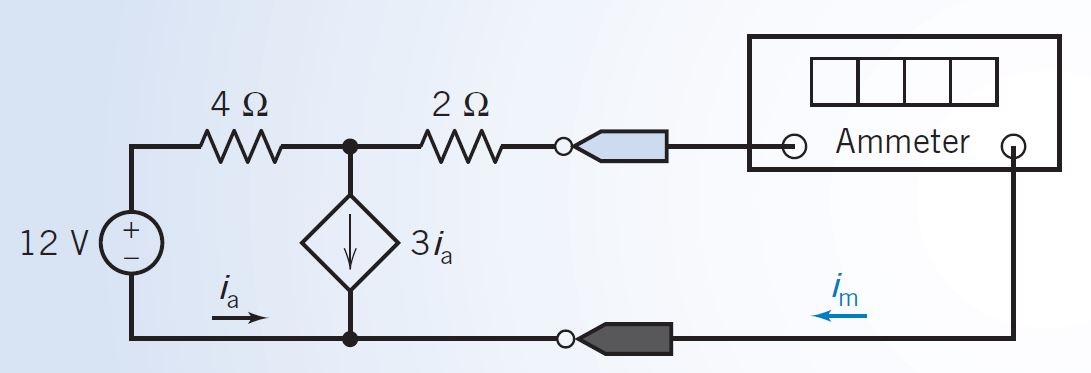
\includegraphics[width=1\textwidth]{figura4.JPG}
     					\end{center}	
				\end{column}
				\begin{column}{0.5\textwidth}  %%<--- here
					\begin{itemize}
						\item[$\clubsuit$] Determine the value of the current, in amps, measured by the ammeter.
					\end{itemize}
				\end{column}
			\end{columns}
		\\
			\begin{columns}[c]
				\column{1\textwidth}

				\textbf{E X A M P L E 3.2-5} -  Ohm’s and Kirchhoff’s Laws
			\end{columns}	
		 \\
			\begin{columns}
				\begin{column}{0.5\textwidth}  %%<--- here
    					\begin{center}	
     						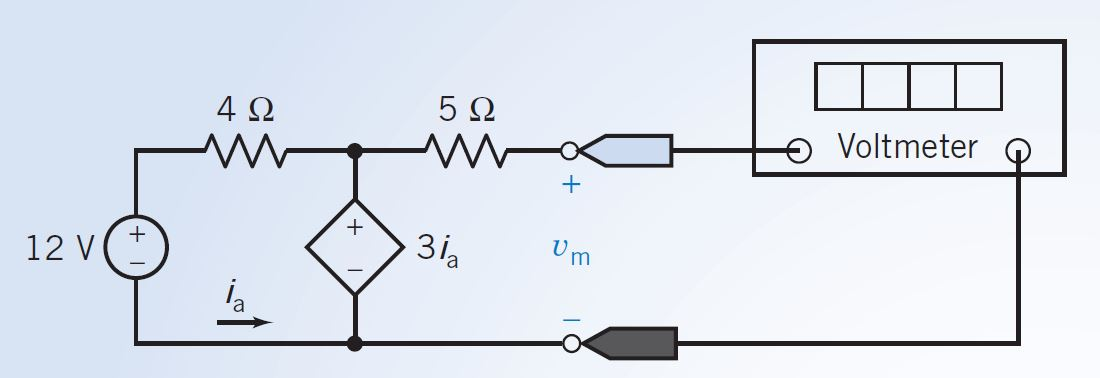
\includegraphics[width=1\textwidth]{figura5.JPG}
     					\end{center}	
				\end{column}
				\begin{column}{0.5\textwidth}  %%<--- here
					\begin{itemize}
						\item[$\clubsuit$] Determine the value of the voltage, in volts, measured by the voltmeter.
					\end{itemize}
				\end{column}
			\end{columns}	
		
   		\end{tabular}
\end{frame}
% ----------------- NOVO SLIDE --------------------------------
\begin{frame}[fragile]
	\frametitle{ Kirchhoff’s Laws}
		\begin{tabular}{ccc}
			\begin{columns}[c]
				\column{1\textwidth}
				\textbf{EXERCISE 3.2-1} -  Determine the values of  $ i_{3}, i_{4}, i_{6}, v_{2}, v_{4}\ and\ v_{6}$.
			\end{columns}
		 \\
			\begin{columns}
				\begin{column}{.8\textwidth}  %%<--- here
    				%	\begin{flushleft}	
     						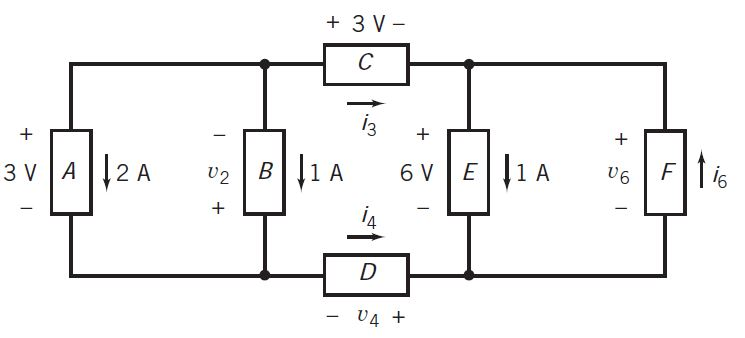
\includegraphics[width=10cm]{figura6.JPG}
     				%	\end{flushleft}	
				\end{column}
			\end{columns}
		

		 \\
			\begin{columns}[c]
				\column{1\textwidth}


				\scalebox{0.8}{Answer:$ i_{3} = -3 A, i_{4} = 3 A, i_{6} = 4 A, v_{3} = -3 V, v_{4}= - 6 V, v_{6}= 6 V$}
			\end{columns}


   		\end{tabular}
\end{frame}
% ----------------- NOVA SECÇÂO -----------------------------
\section{Series Resistors and Voltage Division (3.3)}
% ----------------- NOVO SLIDE --------------------------------
\begin{frame}[fragile]
	\frametitle{Series Resistors and Voltage Division}
		\begin{tabular}{ll}
			\begin{columns}[c]
				\column{1\textwidth}
\\
				Let us consider a single-loop circuit ...
			\end{columns}
		 \\
			\begin{columns}
				\begin{column}{.3\textwidth}  %%<--- here
    					
     					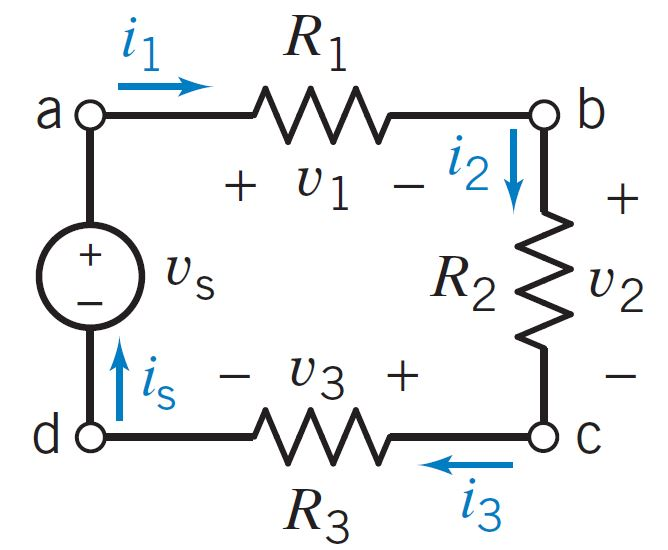
\includegraphics[width=5cm]{figura7.JPG}\\
					\begin{figure}
					{\small Single-loop circuit with a voltage source $ v_{s}$.}
     					\end{figure}	
				\end{column}
				\begin{column}{0.5\textwidth}  %%<--- here
    					%\begin{center}
     						In general, we may represent the voltage divider principle by the equation:
					\begin{equation}
						 v_{n}=\frac{ R_{n} v_{s}}{R_{1} +  R_{2} + ... + R_{N}}
					\end{equation}
						where $v_{n}$ is the voltage across the nth resistor of N resistors connected in series.
     					%\end{center}	
				\end{column}
			\end{columns}
		
	\end{tabular}
\end{frame}

% ----------------- NOVA SECÇÂO -----------------------------
\section{Parallel Resistors and Current Division (3.4)}
% ----------------- NOVO SLIDE --------------------------------



\begin{frame}[fragile]
	\frametitle{Parallel Resistors and Current Division}
		\begin{tabular}{ccc}
			\begin{columns}
				\column{1\textwidth}
				Consider the circuit with N conductors and a current source ...
			\end{columns}
		 \\
			\begin{columns}[c]
				\begin{column}{1\textwidth}  %%<--- here
    			%		\begin{figure}	
     						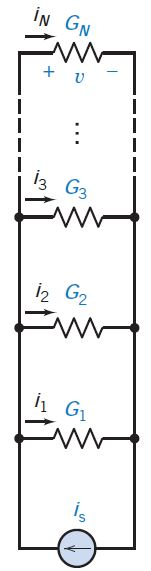
\includegraphics[width=2cm,  angle=-90]{figura8.JPG}
     	%				\end{figure}	
				\end{column}
			\end{columns}
		

		 \\
			\begin{columns}[c]
				\column{1\textwidth}
				In general, we may represent the current divider principle by the equation:
			\begin{equation}
			 i_{n}=\frac{G_{n} i_{s} }{G_{1} +  G_{2} + ... + G_{N}}=\frac{G_{n} i_{s} }{\sum_{k=1}^{N} G_{k}}, where\ G_{n}=\frac{1 }{ R_{n}}
			\end{equation}
			and  $i_{n}$ is the current across the nth conductor of N conductors connected in parallel and $G_{n}$.
			\end{columns}


   		\end{tabular}
\end{frame}

% ----------------- NOVA SECÇÂO -----------------------------
%\section{Equivalent Circuit}
% ----------------- NOVO SLIDE --------------------------------
\begin{frame}[fragile]
	\frametitle{Equivalent Circuit}
		\begin{tabular}{ll}
			\begin{columns}[c]
				\column{1\textwidth}
					\begin{itemize}
						\item[$\clubsuit$] Equivalent circuit for a series resistors
					\end{itemize}
			\end{columns}
		 \\
			\begin{columns}
				\begin{column}{0.5\textwidth}  %%<--- here
    				%	\begin{center}	
     						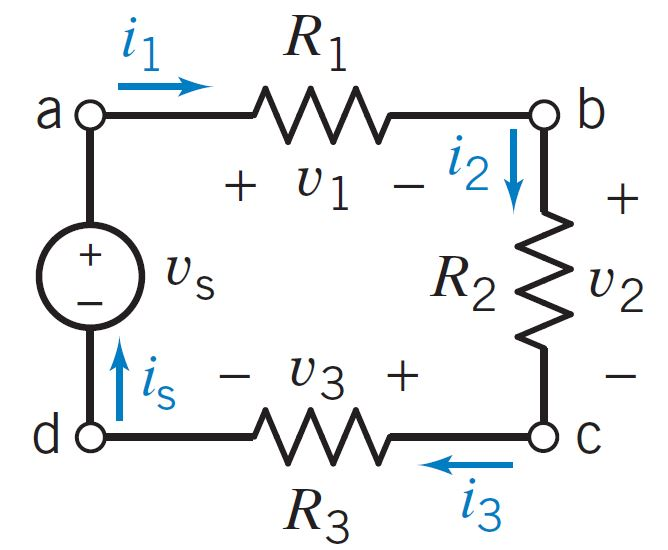
\includegraphics[width=3cm]{figura7.JPG}
=
						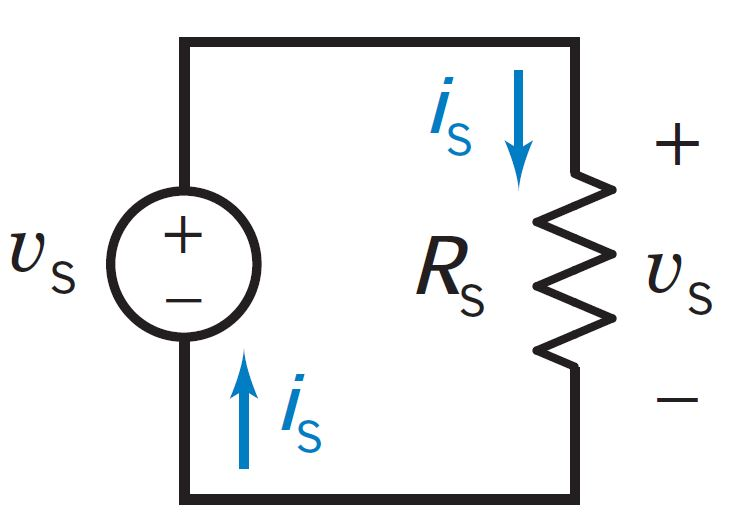
\includegraphics[width=3cm]{figura9.JPG}
     				%	\end{center}	
				\end{column}
				\begin{column}{0.5\textwidth}  %%<--- here
					\begin{equation}
    						 R_{s}= R_{1} +  R_{2} + ... + R_{N}	={\sum_{n=1}^{N} R_{n}}
					\end{equation}
					
				\end{column}
			\end{columns}
		\\
			\begin{columns}[c]
				\column{1\textwidth}
				\begin{itemize}
					\item[$\clubsuit$] Equivalent circuit for a parallel resistors
				\end{itemize}
			\end{columns}	
		 \\
			\begin{columns}
				\begin{column}{0.5\textwidth}  %%<--- here
    				%	\begin{center}	
     						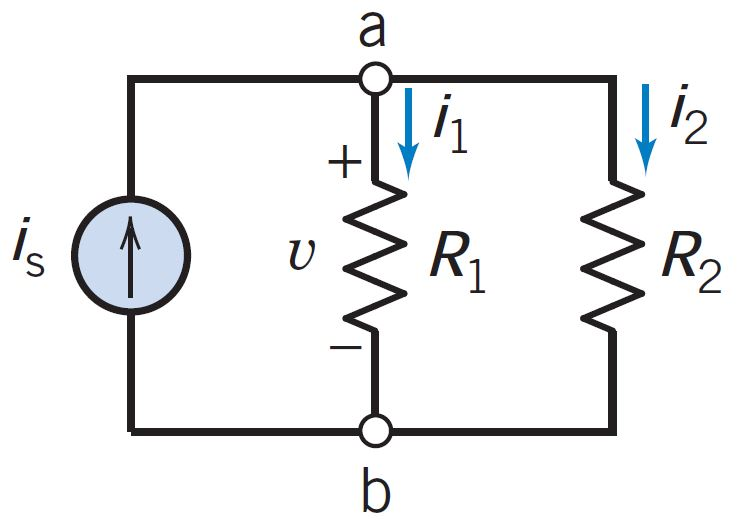
\includegraphics[width=3cm]{figura10.JPG}
=
						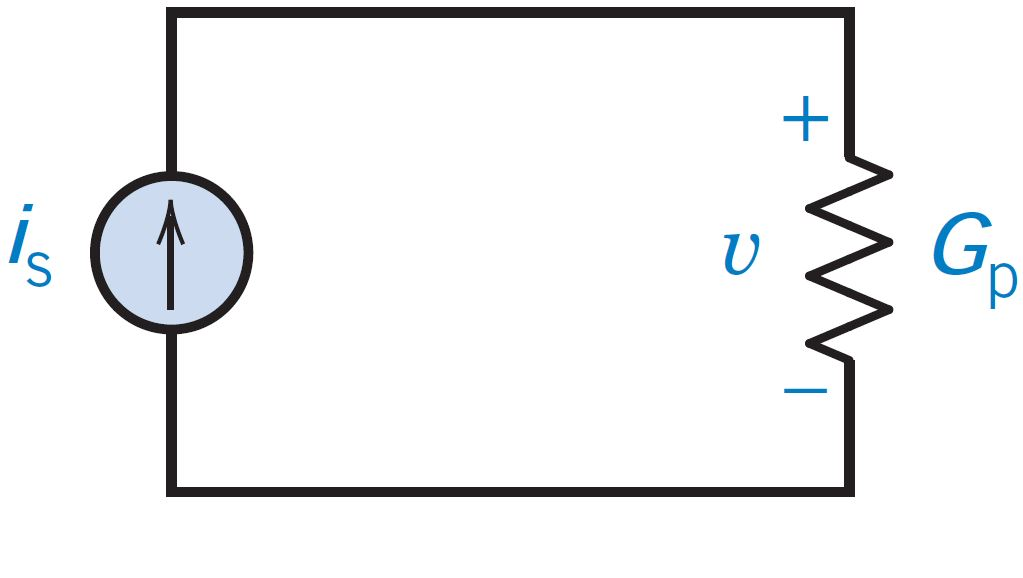
\includegraphics[width=3cm]{figura11.JPG}
     				%	\end{center}	
				\end{column}
				\begin{column}{0.5\textwidth}  %%<--- here
    					\begin{equation}
    						 G_{p}=\frac{1 }{R_{p}}=\frac{1 }{R_{1}}+...+\frac{1 }{R_{N}}={\sum_{n=1}^{N} \frac{1}{R_{n}}}
					\end{equation}
					
				\end{column}
			\end{columns}	
		
   		\end{tabular}
\end{frame}
% ----------------- NOVA SECÇÂO -----------------------------
\section{Series Voltage Sources and Parallel Current Sources (3.5)}
% ----------------- NOVO SLIDE --------------------------------
\begin{frame}[fragile]
	\frametitle{Series Voltage Sources}
		\begin{tabular}{ll}
	%		\begin{columns}[c]
	%			\column{1\textwidth}
				
	
	%		\end{columns}
	%	 \\
			\begin{columns}
				\begin{column}{0.5\textwidth}  %%<--- here
    				%	\begin{center}
						Voltage sources connected in series are equivalent to a single voltage source. 
     						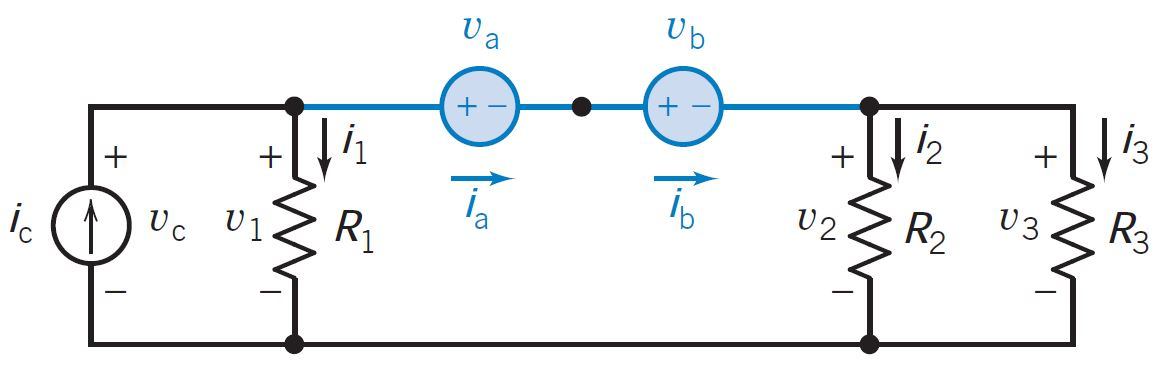
\includegraphics[width=6cm]{figura12.JPG}
						\\
						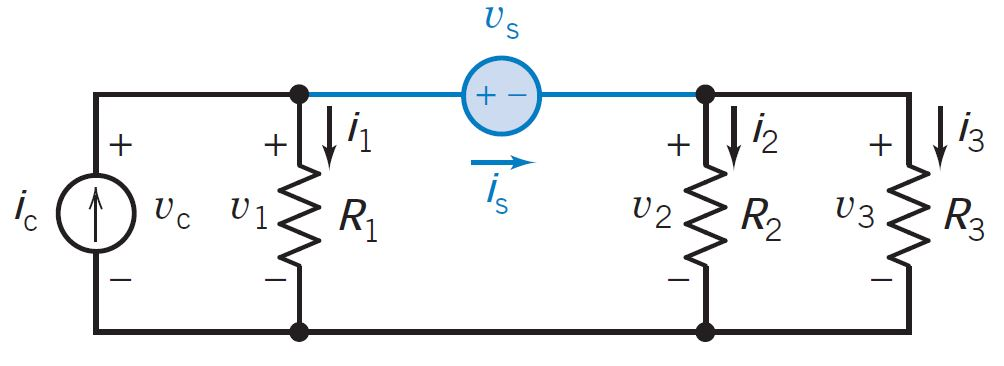
\includegraphics[width=6cm]{figura13.JPG}\\
     				%	\end{center}	
				\end{column}
				\begin{column}{0.5\textwidth}  %%<--- here
				%	\begin{center}	
     						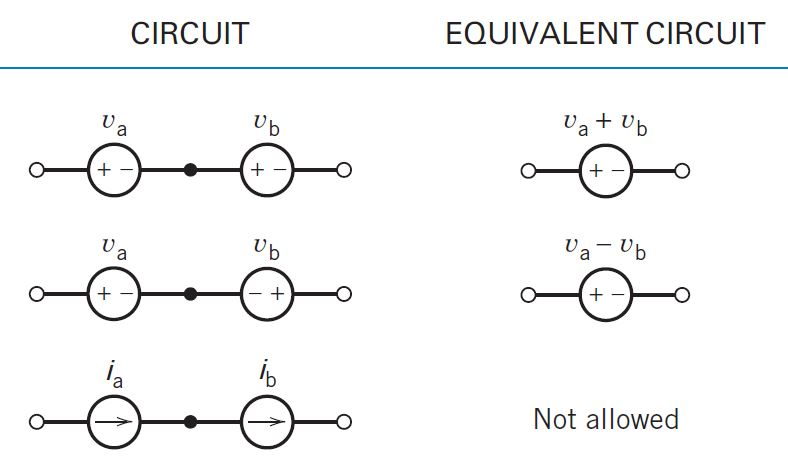
\includegraphics[width=7cm]{figura14.JPG}
				%	\end{center}				
				\end{column}
			\end{columns}
		\end{tabular}
\end{frame}
% ----------------- NOVA SECÇÂO -----------------------------
%\section{Parallel Current Sources}
% ----------------- NOVO SLIDE --------------------------------
\begin{frame}[fragile]
	\frametitle{Parallel Current Sources}
		\begin{tabular}{ll}
			\begin{columns}
				\begin{column}{0.5\textwidth}  %%<--- here
    					\begin{center}
						Equivalent current source is equal to the algebraic sum of the currents of the parallel current sources. 
     						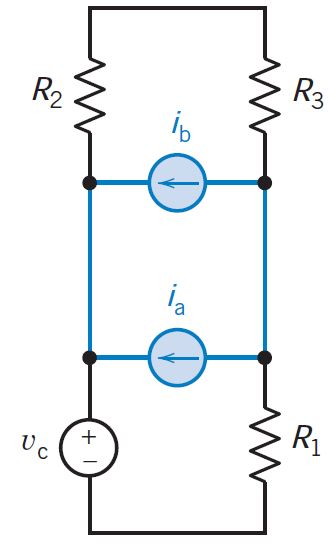
\includegraphics[width=3cm]{figura16.JPG}\
						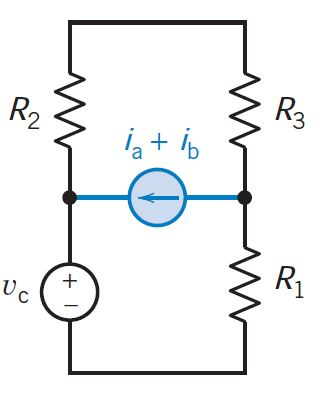
\includegraphics[width=3cm]{figura17.JPG}
     					\end{center}	
				\end{column}
				\begin{column}{0.5\textwidth}  %%<--- here
					\begin{center}	
     						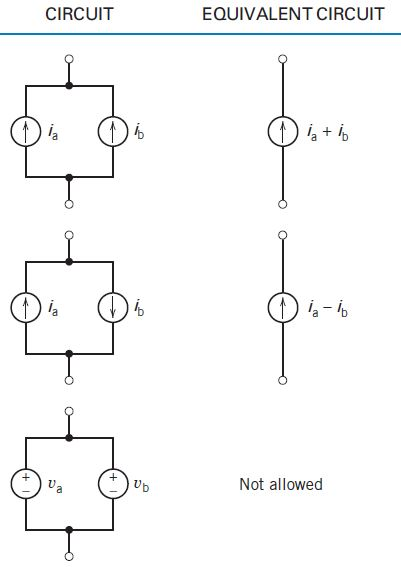
\includegraphics[width=4.5cm]{figura15.JPG}
					\end{center}				
				\end{column}
			\end{columns}
		\end{tabular}
\end{frame}
% ----------------- NOVO SLIDE --------------------------------
\begin{frame}[fragile]
	\frametitle{Series and Parallel Sources}
		\begin{tabular}{ll}
			\begin{columns}[c]
				\column{1\textwidth}
				\textbf{E X A M P L E 3.5-1a} -  Show similar circuits
			\end{columns}
		 \\
			\begin{columns}
				\begin{column}{0.5\textwidth}  %%<--- here
    					\begin{center}	
     						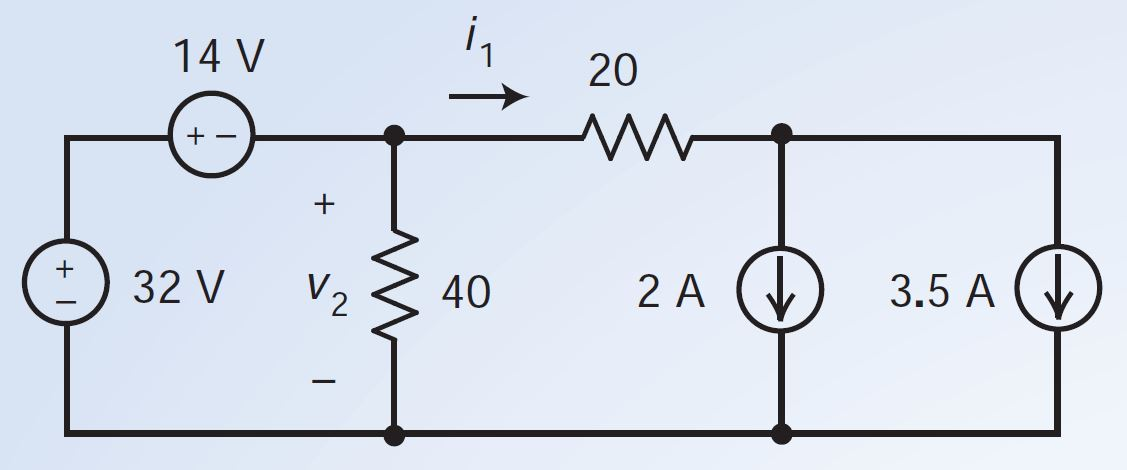
\includegraphics[width=.8\textwidth]{figura18.JPG}
     					\end{center}	
				\end{column}
				\begin{column}{0.5\textwidth}  %%<--- here
					\begin{itemize}
						\item[$\clubsuit$] Determine the value of the current $i_{1}$ and voltage $v_{2}$.
					\end{itemize}
				\end{column}
			\end{columns}
		\\
			\begin{columns}[c]
				\column{1\textwidth}

				\textbf{E X A M P L E 3.5-1c} -   Show similar circuits
			\end{columns}	
		 \\
			\begin{columns}
				\begin{column}{0.5\textwidth}  %%<--- here
    					\begin{center}	
     						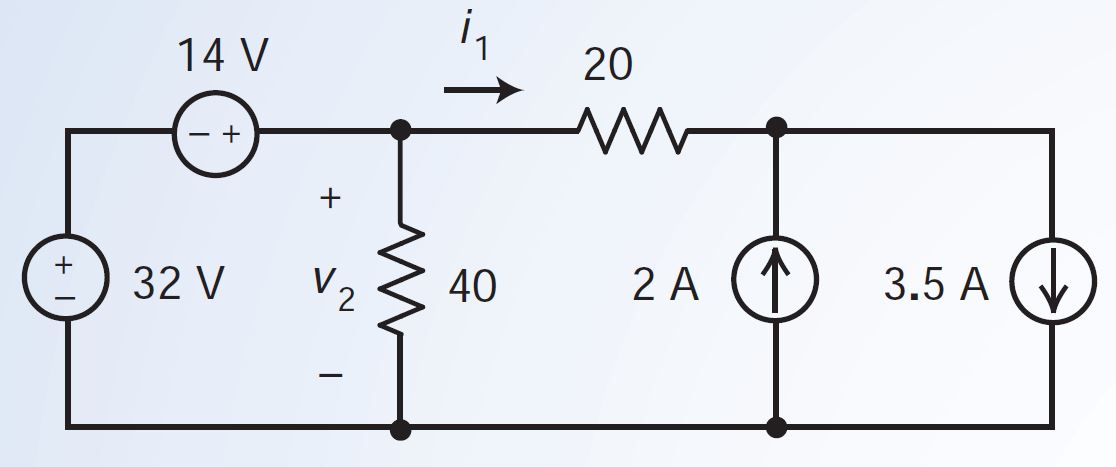
\includegraphics[width=.8\textwidth]{figura19.JPG}
     					\end{center}	
				\end{column}
				\begin{column}{0.5\textwidth}  %%<--- here
					\begin{itemize}
						\item[$\clubsuit$] Determine the value of the current $i_{1}$ and voltage $v_{2}$.
					\end{itemize}
				\end{column}
			\end{columns}	
		
   		\end{tabular}
\end{frame}


% ----------------- NOVA SECÇÂO -----------------------------
\section{Circuit Analysis (3.6)}
% ----------------- NOVO SLIDE --------------------------------
\begin{frame}[fragile]
	\frametitle{Analyzing Resistive Circuits}
		\begin{tabular}{ll}
			\begin{columns}
				\begin{column}{0.5\textwidth}  %%<--- here
\begin{tabular}{ll}    					
%\begin{figure}	
     						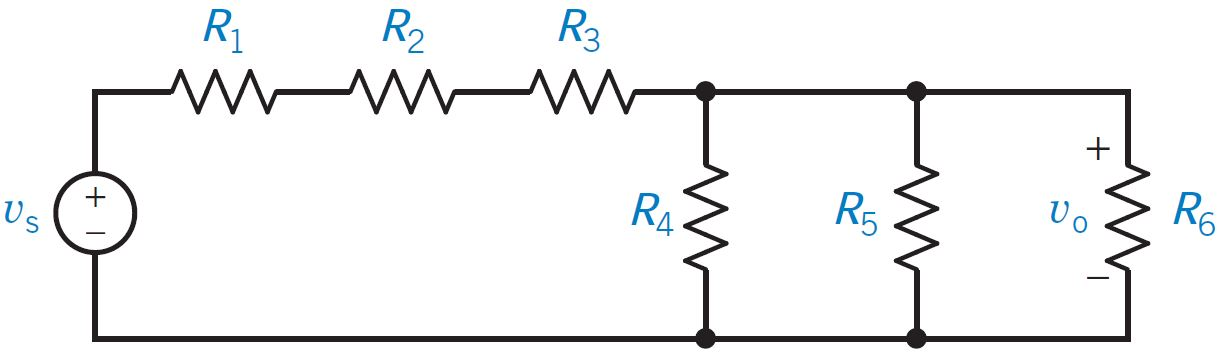
\includegraphics[width=8cm]{figura20.JPG}\\
						{( a ) Set of series and parallel resistors.}\\
						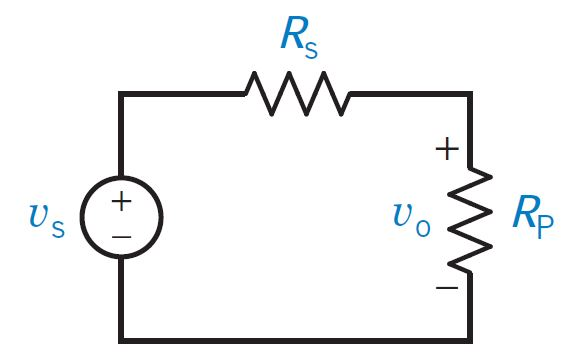
\includegraphics[width=4cm]{figura21.JPG}\\
						{( b ) Equivalent circuit. }
     					%\end{figure}
\end{tabular}	
				\end{column}
				\begin{column}{0.5\textwidth}  %%<--- here
      					\begin{equation}
    						 R_{s}= R_{1} +  R_{2} + R_{3}
					\end{equation}
					\begin{equation}
    						 R_{p}=\frac{1 }{G_{p}}
					\end{equation}
					\begin{equation}
    						 R_{s}= R_{1} +  R_{2} + R_{3}
					\end{equation}
					\begin{equation}
    						 v_{o}=\frac{R_{p}}{R_{s}+R_{p}} v_{s}
					\end{equation}\\	
					The analysis of a circuit by replacing a set of resistors with an equivalent
					resistance, thus reducing the network to a form easily analyzed.	
				\end{column}
			\end{columns}
		\end{tabular}
\end{frame}
% ----------------- NOVO SLIDE --------------------------------
\begin{frame}[fragile]
	\frametitle{ Analyzing Resistive Circuits}
		\begin{tabular}{ccc}
			\begin{columns}
				\begin{column}{.4\textwidth}  %%<--- here
    					\begin{figure}
     						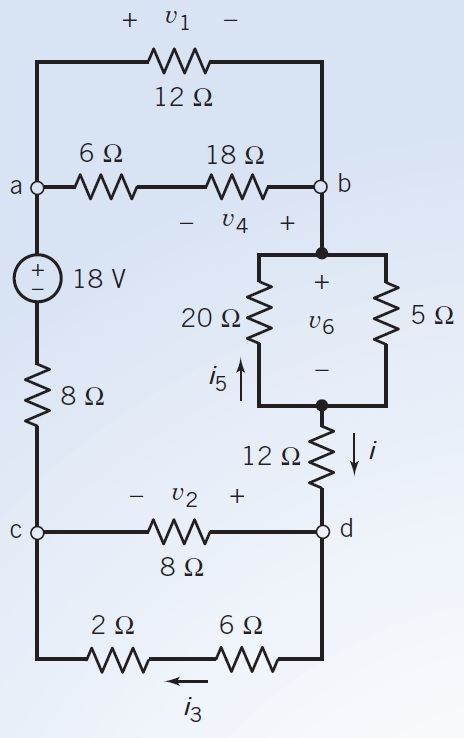
\includegraphics[width=3.5cm]{figura22.JPG}
     					\end{figure}	
				\end{column}
				\begin{columns}[c]
					\column{1\textwidth}
					\textbf{EXEMPLE 3.6-3} -  Determine the values of  $ i_{3}, v_{4}, i_{5}\ and\ v_{6}$.\\
					\scalebox{0.8}{Answer:$ i_{3} = 0.25 A, v_{4} = -3 V, i_{5} = -0.1 A, v_{6} = 2 V$}
				\end{columns}
			\end{columns}
		

		 \\



   		\end{tabular}
\end{frame}

% ----------------- NOVA SECÇÂO -----------------------------
\section{Analyzing Resistive Circuits Using MATLAB}
% ----------------- NOVO SLIDE --------------------------------
\begin{frame}[fragile]
	\frametitle{ Analyzing Resistive Circuits Using MATLAB}
		\begin{tabular}{ccc}
			\begin{columns}[c]
				\column{1\textwidth}
				\textbf{EXERCISE 3.7-1} -  Determine the values of the resistor voltages and currents.
			\end{columns}
		 \\
			\begin{columns}
				\begin{column}{.8\textwidth}  %%<--- here
    				%	\begin{flushleft}	
     						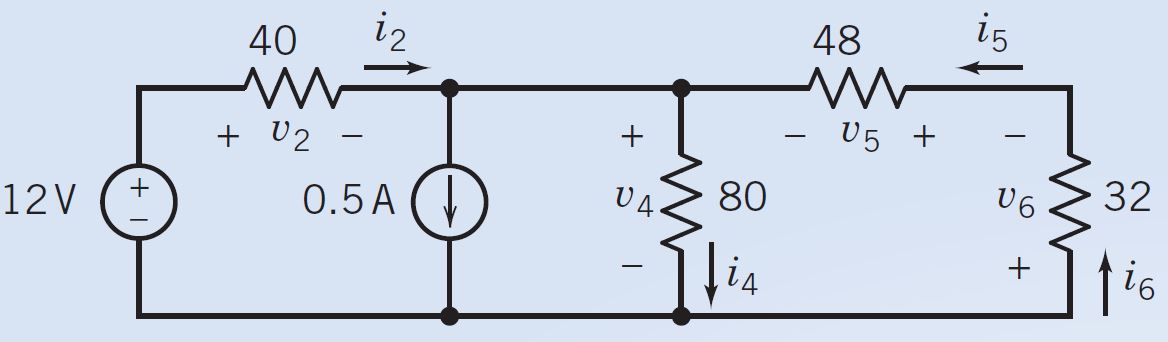
\includegraphics[width=10cm]{figura23.JPG}
     				%	\end{flushleft}	
				\end{column}
			\end{columns}
		

		 \\
			\begin{columns}[c]
				\column{1\textwidth}

			\scalebox{0.8}{Answer:$ i_{2} = 0.4 A, i_{4} = -0.05 A, i_{5} = 0.05 A, i_{6}= 0.05 A, v_{2}= 16 V, v_{4}= -4 V, v_{5}= 2.4 V\ and \ v_{6}= 1.6 V$}
			\end{columns}


   		\end{tabular}
\end{frame}



\end{document} 